\section{Analysis}
\label{sec:Analysis}
The decay $\text{B}^{\pm} \to K^{+} \, K^{-} \, K^{\pm}$ is reconstructed from data recorded by the LHCb experiment in 2011.
First,
particle identification information is used to suppress background
from misidentified final-state particles, and the invariant mass of the
reconstructed $B$ meson candidates is used to isolate the signal.
This is described in \autoref{sec:Preselection}.
The global CP asymmetry is then studied in \autoref{sec:Global} using the preselected data.
The two-body resonances are subsequently investigated in \autoref{sec:Resonanz},
after which the resonance contributions are removed and the local CP asymmetry is examined in \autoref{sec:Local}.

\subsection{Preselection}
\label{sec:Preselection}
In order to isolate genuine $B^{\pm} \rightarrow K^{\pm}K^{+}K^{-}$ decays,
a preselection is applied to suppress background contributions arising from the misidentification of the three final-state particles.
Two sources of such background are considered.
First,
muons are explicitly removed from the sample.
Second, particle identification (PID) information provided by the LHCb
detector is used to discriminate between kaons and pions.
For each final-state hadron $i \in \{1,2,3\}$,
a requirement is imposed on the probability of the
hadron being a kaon,
$\mathrm{ProbK}_i$,
and on the probability of it being a
pion,
$\mathrm{ProbPi}_i$:
\begin{align}
    \mathrm{H}i\_\mathrm{ProbK} &> 0.5, \\
    \mathrm{H}i\_\mathrm{ProbPi} &< 0.5.
\end{align}

The distributions of $\mathrm{ProbK}$ and $\mathrm{ProbPi}$ for the three final-state hadrons after the preselection are shown in \autoref{fig:PID}.
\begin{figure}[htbp]
    \centering
    \begin{subfigure}[b]{0.48\textwidth}
        \centering
        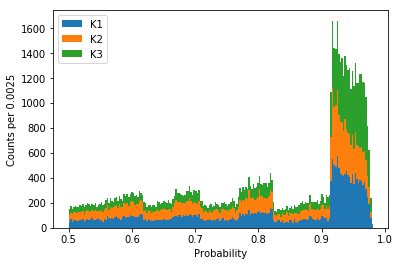
\includegraphics[width=\textwidth]{plots/PID_Kaon.png}
        \caption{Distribution of $\mathrm{ProbK}$.}
        \label{fig:probK}
    \end{subfigure}
    \hfill
    \begin{subfigure}[b]{0.48\textwidth}
        \centering
        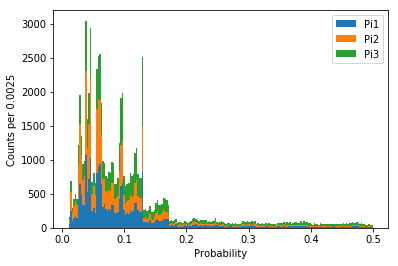
\includegraphics[width=\textwidth]{plots/PID_Pion.png}
        \caption{Distribution of $\mathrm{ProbPi}$.}
        \label{fig:probPi}
    \end{subfigure}
    \caption{One-dimensional particle identification distributions for the
    three final-state hadrons: (a) probability of (K1, K2, K3) being a kaon, and
    (b) probability of (Pi1, Pi2, Pi3) being a pion.}
    \label{fig:PID}
\end{figure}
The preselection effectively suppresses background from misidentified particles.
A pronounced pion peak is visible at $\mathrm{ProbPi} \lesssim 10\%$ in \autoref{fig:probPi};
rejecting this region entirely would,
however,
result in a substantial loss of signal efficiency and was therefore avoided.
The same argument applies to the $\mathrm{ProbK}$ distribution:
retaining only candidates within the narrow kaon peak would discard a significant fraction of genuine signal events,
and a moderate selection threshold was preferred.

With the preselection applied,
the invariant mass of the reconstructed $B$ meson candidates is calculated from the energy and momentum of the three final-state hadrons,
using the known kaon mass of $493.677\,\text{MeV}$ \cite{PDG2024}.
The resulting invariant mass distribution is shown in \autoref{fig:invariant_mass}.
\begin{figure}[htbp]
    \centering
    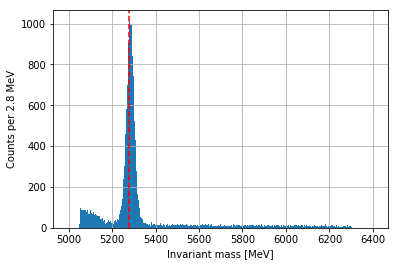
\includegraphics[width=0.6\textwidth]{plots/invariant_mass.png}
    \caption{Invariant mass distribution of the reconstructed $B$ meson candidates after the preselection.
             The red line indicates the known $B$ meson mass of $5279.34\,\text{MeV}$ \cite{PDG2024}.}
    \label{fig:invariant_mass}
\end{figure}
To isolate the signal,
all candidates with an invariant mass between $5220\,\text{MeV}$ and $5350\,\text{MeV}$ are retained,
as shown in \autoref{fig:invariant_mass_cut}.
\begin{figure}[htbp]
    \centering
    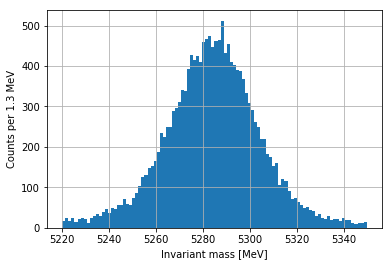
\includegraphics[width=0.6\textwidth]{plots/invariant_mass_cut.png}
    \caption{Invariant mass distribution of the reconstructed $B$ meson candidates after the signal window selection.}
    \label{fig:invariant_mass_cut}
\end{figure}



\subsection{Global CP asymmetry}
\label{sec:Global}
To study the global CP asymmetry,
the $B^{+}$ and $B^{-}$ candidates are distinguished using the charge information of the final-state kaons.
The CP asymmetry is defined as
\begin{equation}
    A_{CP} = \frac{N(B^{+}) - N(B^{-})}{N(B^{+}) + N(B^{-})}
    \label{eq:Aq}
\end{equation}
where $N(B^{+})$ and $N(B^{-})$ denote the number of reconstructed $B^{+}$ and $B^{-}$ candidates, respectively.
The observed yields are
\begin{align}
    N(B^{+}) &=  8651, \\
    N(B^{-}) &=  7842.
\end{align}
Inserting these into \autoref{eq:Aq} yields a global CP asymmetry of
\begin{equation}
    A_{CP} = 0.049 \pm 0.007.
\end{equation}
The statistical significance of this result is
\begin{equation}
    \mathcal{S} = \frac{A_{CP}}{\sigma_{A_{CP}}} = 6.3.
\end{equation}



\subsection{Two-body resonances}
\label{sec:Resonanz}
The decay $B^{+} \rightarrow K^{+}_{1}K^{+}_{2}K^{-}_{3}$ can proceed either directly to the three-body final state or via an intermediate resonance,
for example $B^{+} \rightarrow K^{+}R^{0}$,
with the subsequent decay $R^{0} \rightarrow K^{+}K^{-}$.
Such intermediate resonances can be identified using a Dalitz plot.

As the kinematics of a three-body decay are fully determined by energy and momentum conservation,
the decay can be described using only two independent variables.
These are chosen to be the squared invariant masses of two of the three possible pairs of final-state particles.
For the decay $B^{+} \rightarrow K^{+}_{1}K^{+}_{2}K^{-}_{3}$, three two-body pairings can be formed:
$R^{0}_{13} \rightarrow K^{+}_{1}K^{-}_{3}$,
$R^{++}_{12} \rightarrow K^{+}_{1}K^{+}_{2}$,
and $R^{0}_{23} \rightarrow K^{+}_{2}K^{-}_{3}$.
Since mesons consist of a quark-antiquark pair,
their net charge cannot exceed one unit;
the doubly charged combination $R^{++}_{12}$ therefore cannot correspond to a physical resonance and is excluded from further consideration.
The two remaining neutral combinations are used as
the Dalitz plot variables.
Figure~\ref{fig:dalitz} shows the resulting Dalitz plot.
\begin{figure}[htbp]
    \centering
    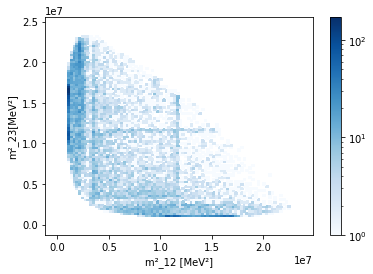
\includegraphics[width=0.6\textwidth]{plots/dalitz.png}
    \caption{Dalitz plot of the decay $B^{+} \rightarrow K^{+}_{1}K^{+}_{2}K^{-}_{3}$.
             The axes correspond to the squared invariant masses of the two neutral two-body combinations of final-state particles.}
    \label{fig:dalitz}
\end{figure}
To improve the visibility of the resonances,
the two neutral combinations are sorted such that $R^0_\text{high}$ denotes the pair with the higher squared invariant mass and $R^0_\text{low}$ the one with the lower value.
This folded Dalitz plot is shown in \autoref{fig:dalitz_folded}.
\begin{figure}
    \centering
    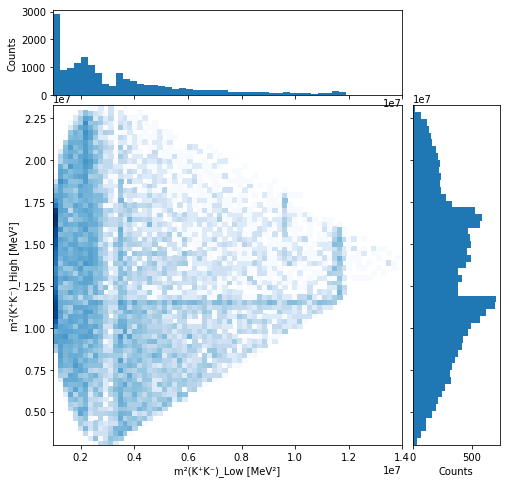
\includegraphics[width=0.6\textwidth]{plots/dalitz_folded.png}
    \caption{Folded Dalitz plot with one-dimensional projections along each axis to facilitate the identification of resonance bands.}
    \label{fig:dalitz_folded}
\end{figure}
A resonance band at
\[
m^2 \approx 1.17\times10^{7}\,\text{MeV}^2
\]
is clearly visible.  
This corresponds to the $\chi_{c0}$ resonance, which has a rest-frame mass of
$3414.71\,\text{MeV}$ \cite{PDG2024} and can decay into a pair of kaons.

A second possible resonance band is observed at
\[
m^2 \approx 3.45\times10^{6}\,\text{MeV}^2.
\]
However, this structure cannot be attributed to a known resonance decaying into two kaons in this mass region and is therefore likely of non-resonant or combinatorial origin.

A third possible resonance band is observed at
\[
m^2 \approx 9.69\times10^{6}\,\text{MeV}^2.
\]
This is consistent with the $J/\psi$ resonance, which has a rest-frame mass of
$3096.916\,\text{MeV}$ \cite{PDG2024}. Although the $J/\psi(1S)$ does not decay directly into two kaons with a large branching fraction, it can contribute via misidentification or rare decay channels.

The Dalitz plot with the vetoed resonance regions is shown in \autoref{fig:dalitzcut}.
\begin{figure}
	\centering
	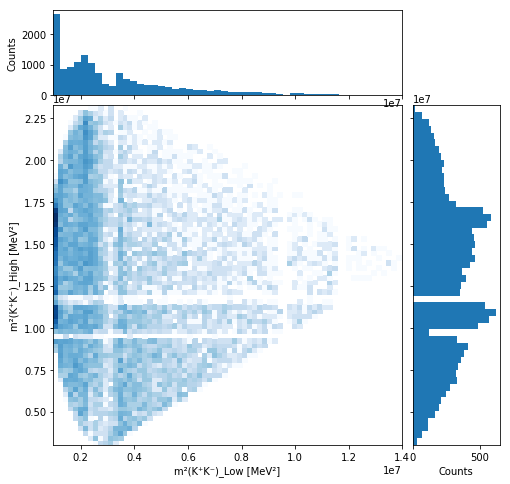
\includegraphics[width=0.6\textwidth]{plots/dalitz_cut.png}
	\caption{Folded Dalitz plot with one-dimensional projections along each axis .mThe $\chi_{c0}$  resonance is cut out. }
	\label{fig:dalitzcut}
\end{figure}



\subsection{Local CP asymmetry}
\label{sec:Local}
To study the local CP asymmetry, the $\chi_{c0}$ resonance identified in \autoref{sec:Resonanz} is removed from the dataset.
Separate Dalitz plots are then constructed for the $B^+$ and $B^-$ decay modes,
as shown in \autoref{fig:BB}.
\begin{figure}[htbp]
    \centering
    \begin{subfigure}[b]{0.48\textwidth}
        \centering
        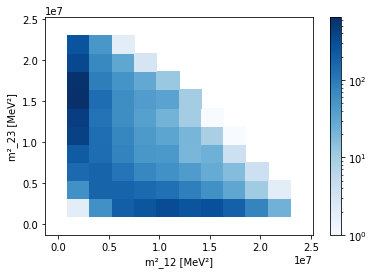
\includegraphics[width=\textwidth]{plots/Bp.png}
        \caption{Dalitz plot for the $B^+$ decay.}
        \label{fig:Bp}
    \end{subfigure}
    \hfill
    \begin{subfigure}[b]{0.48\textwidth}
        \centering
        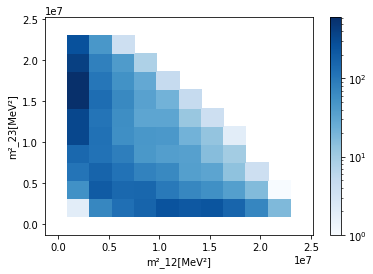
\includegraphics[width=\textwidth]{plots/Bm.png}
        \caption{Dalitz plot for the $B^-$ decay.}
        \label{fig:Bm}
    \end{subfigure}
    \caption{Dalitz plots for the $B^+$ and $B^-$ decays after removal of the $\chi_{c0}$ resonance.}
    \label{fig:BB}
\end{figure}
A coarse binning scheme is employed to ensure sufficient statistical yields per bin.

Applying \autoref{eq:Aq} to each bin of the $B^{\pm}$ Dalitz plots yields the CP asymmetry as a function of phase space,
as shown in \autoref{fig:CP}.
\begin{figure}
    \centering
    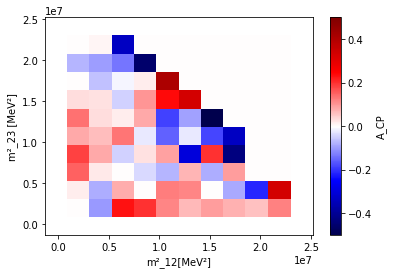
\includegraphics[width=0.6\textwidth]{plots/CP.png}
    \caption{Bin-by-bin CP asymmetry $A_{CP}$ across the Dalitz plot phase space after removal of the $\chi_{c0}$ resonance.}
    \label{fig:CP}
\end{figure}
To identify regions of significant local CP violation, the statistical uncertainty ($\sigma$) and significance are determined for each bin,
as shown in \autoref{fig:unsicher}.
\begin{figure}[htbp]
    \centering
    \begin{subfigure}[b]{0.48\textwidth}
        \centering
        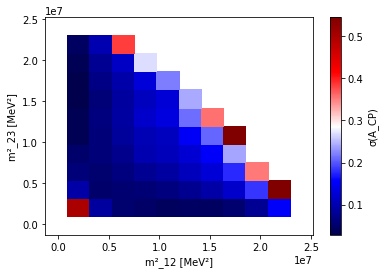
\includegraphics[width=\textwidth]{plots/uns.png}
        \caption{Statistical uncertainty $\sigma_{A_{CP}}$.}
    \end{subfigure}
    \hfill
    \begin{subfigure}[b]{0.48\textwidth}
        \centering
        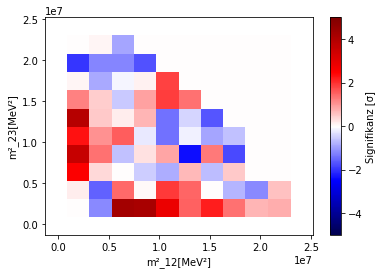
\includegraphics[width=\textwidth]{plots/sig.png}
        \caption{Significance $\mathcal{S} = A_{CP}/\sigma_{A_{CP}}$.}
    \end{subfigure}
    \caption{Bin-by-bin statistical uncertainty and significance of the CP asymmetry between the $B^+$ and $B^-$ Dalitz plots.}
    \label{fig:unsicher}
\end{figure}
Based on the bin-by-bin significance map shown in \autoref{fig:unsicher},
a contiguous region of significant CP violation was identified in the range $0.0 \times 10^{7} < m^{2}(K^{+}K^{-})_{1} < 0.5 \times 10^{ 7}~\text{MeV}^{2}$ and $0.5 \times 10^{7} < m^{2}(K^{+}K^{-})_{2} < 1.7 \times 10^{7}~\text{MeV}^{2}$.
This region exhibits
the largest local CP asymmetry observed across the Dalitz plot and was
therefore selected for further study.

The invariant mass distributions of the $B^+$ and $B^-$ candidates within this selected phase-space region are compared in \autoref{fig:ende}.
\begin{figure}
    \centering
    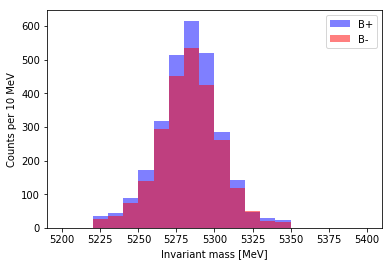
\includegraphics[width=0.6\textwidth]{plots/ende.png}
    \caption{Comparison of the invariant mass distributions for the $B^+$ and $B^-$ decays in the selected phase-space region.}
    \label{fig:ende}
\end{figure}
The $B^+$ yield clearly exceeds that of $B^-$ in this region,
providing evidence for local CP violation. 
The local asymmetry in this region is 
\begin{equation}
	A_\text{CP local} = 0.072 \pm 0.008
\end{equation}
 which is significantly higher than the observed global asymmetry.
